\subsection{Resultados}

    \subsubsection{Valor de RTO variando $\alpha$ y $\beta$}
        Los resultados de medir el \rto{} para un valor fijo de 
        \textit{25 ticks} y probabilidad de perdida cero luego de 
        enviar 200 paquetes se pueden ver en la \emph{Figura 1}.
        
    \subsubsection{Perdida de paquetes variando $\alpha$ y $\beta$}
        Para estudiar la perdida de paquetes se fij\'o el valor de 
        de \rto{} en \textit{25 ticks} y no se simularon p\'erdidas.
        Sin embargo en varios casos hubo retransmisiones, la 
        \textit{Figura 2} muestra el resultado para el env\'io de 150
        paquetes mientras que la \textit{Figura 3} lo muestra para 300.
        
    \begin{figure}[H]
	    \center
	    \begin{subfigure}{0.32\textwidth}
		    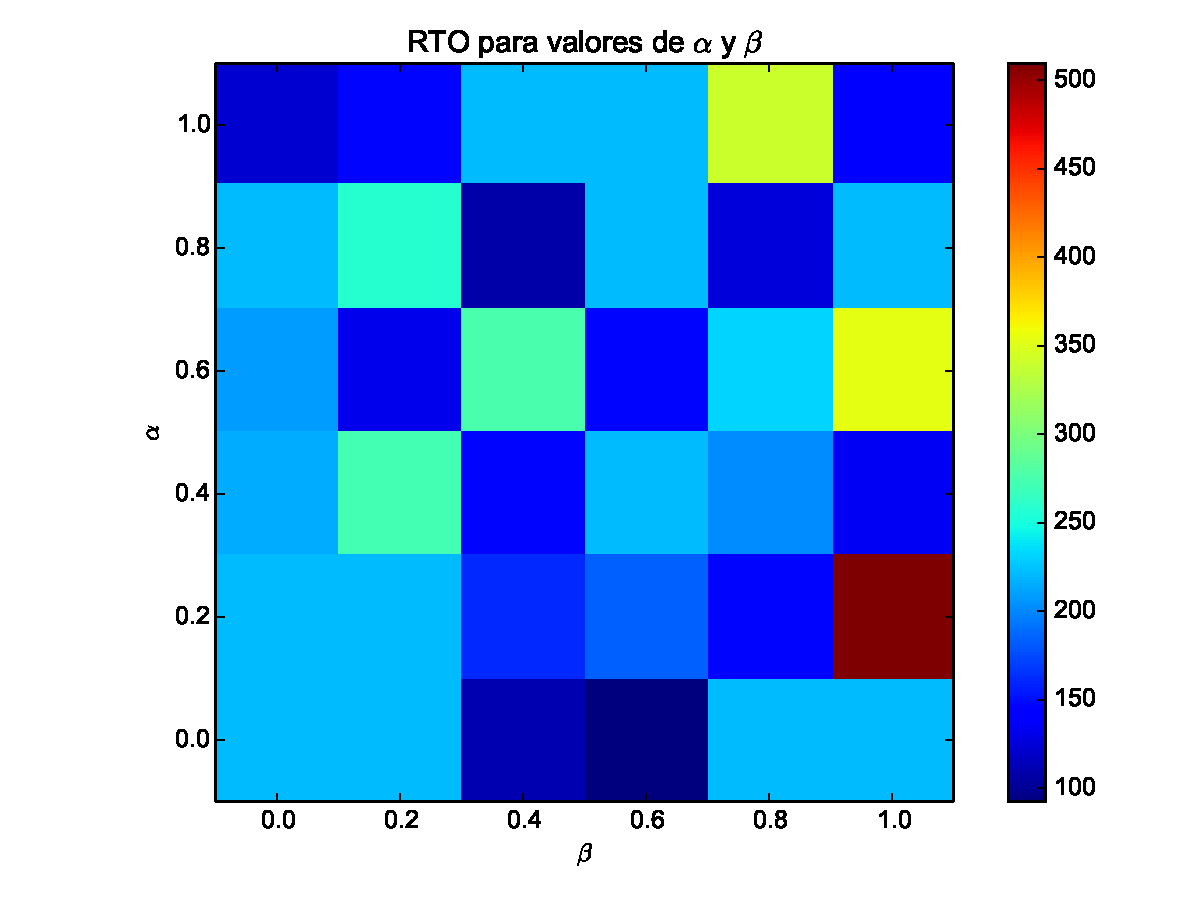
\includegraphics[width=1.0\textwidth]{imagenes/guille/rto_vs_alphaBeta.pdf}
		    \caption{Figura 1}
	    \end{subfigure}
	    ~
	    \begin{subfigure}{0.32\textwidth}
		    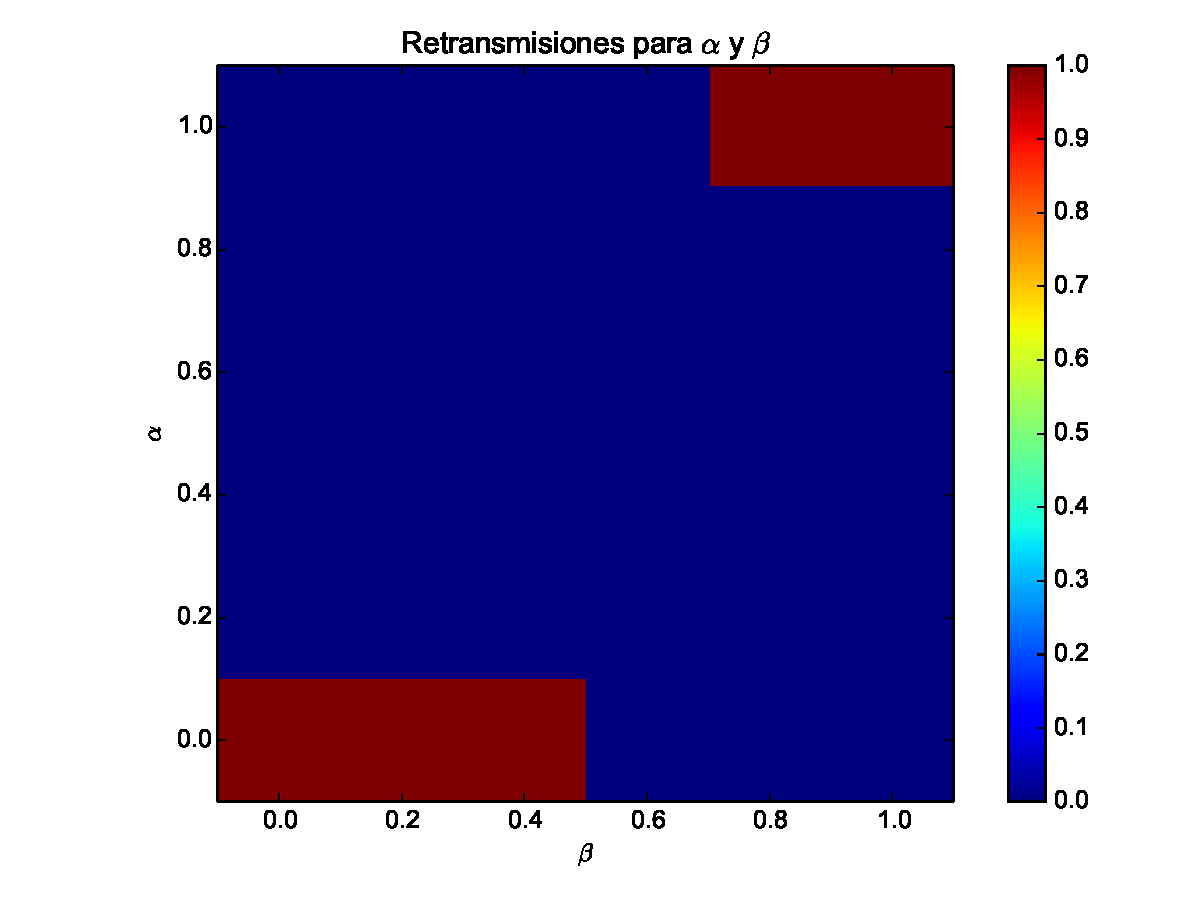
\includegraphics[width=1.0\textwidth]{imagenes/guille/retransmisiones_150.pdf}
		    \caption{Figura 2}
	    \end{subfigure}
	    ~
	    \begin{subfigure}{0.32\textwidth}
		    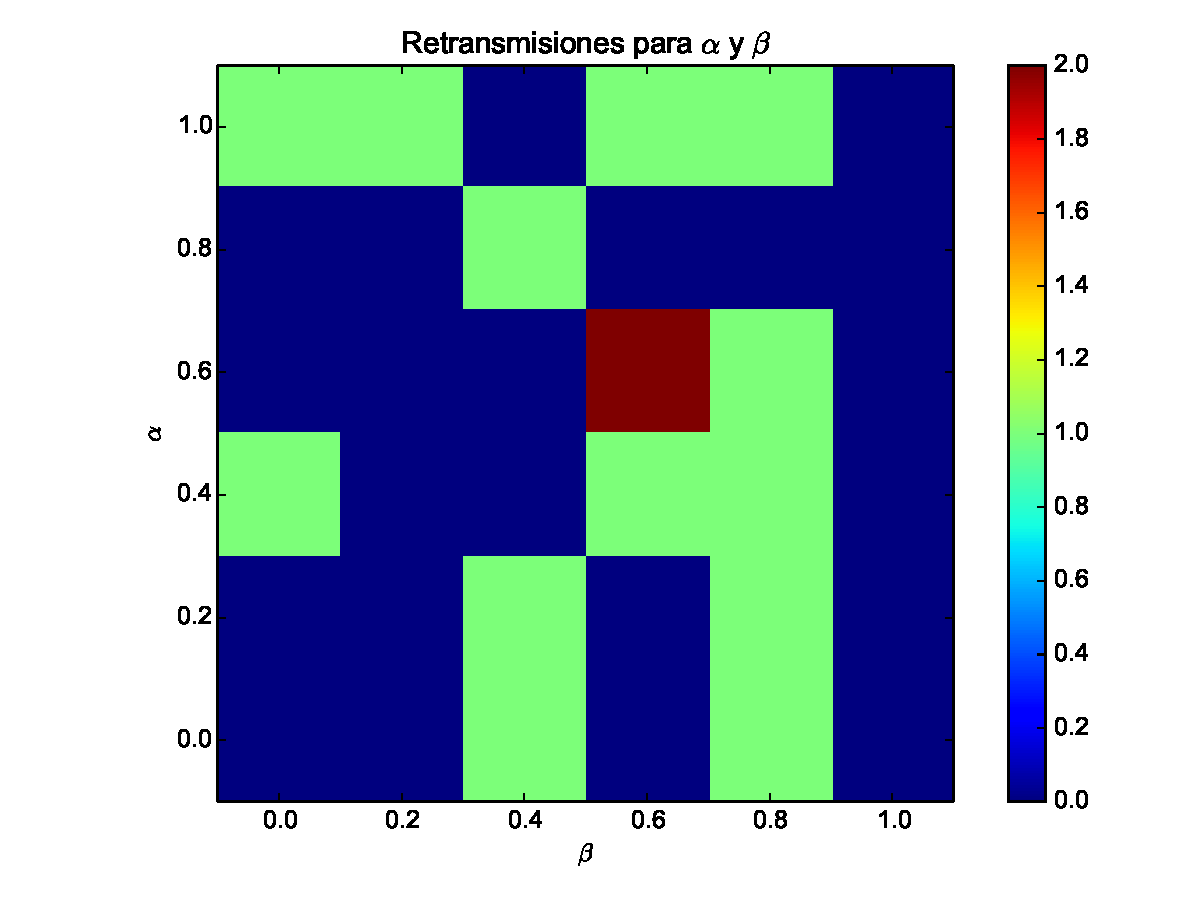
\includegraphics[width=1.0\textwidth]{imagenes/guille/retransmisiones_300.pdf}
		    \caption{Figura 3}
	    \end{subfigure}
	
    \end{figure}    


    \subsubsection{Valor de RTO cuando la red se congestiona sin perdida}
        Para este configuramos el cliente para que env\'ie 300 paquetes al
        servidor, pero luego de enviarse 150 paquetes, el delay de la red
        se duplicara o cuadruplicara. 
        
        El \emph{Escenario 1} muestra el resultado en una red con
        par\'aemtros: $\alpha={{1}\over{2}}$, $\beta={{1}\over{4}}$
        cuando no se congestiona, cuando la congesti\'on causa el doble de
        delay, y cuando causa el cuadruple.
  
        \begin{figure}[H]
            \center
	        
		    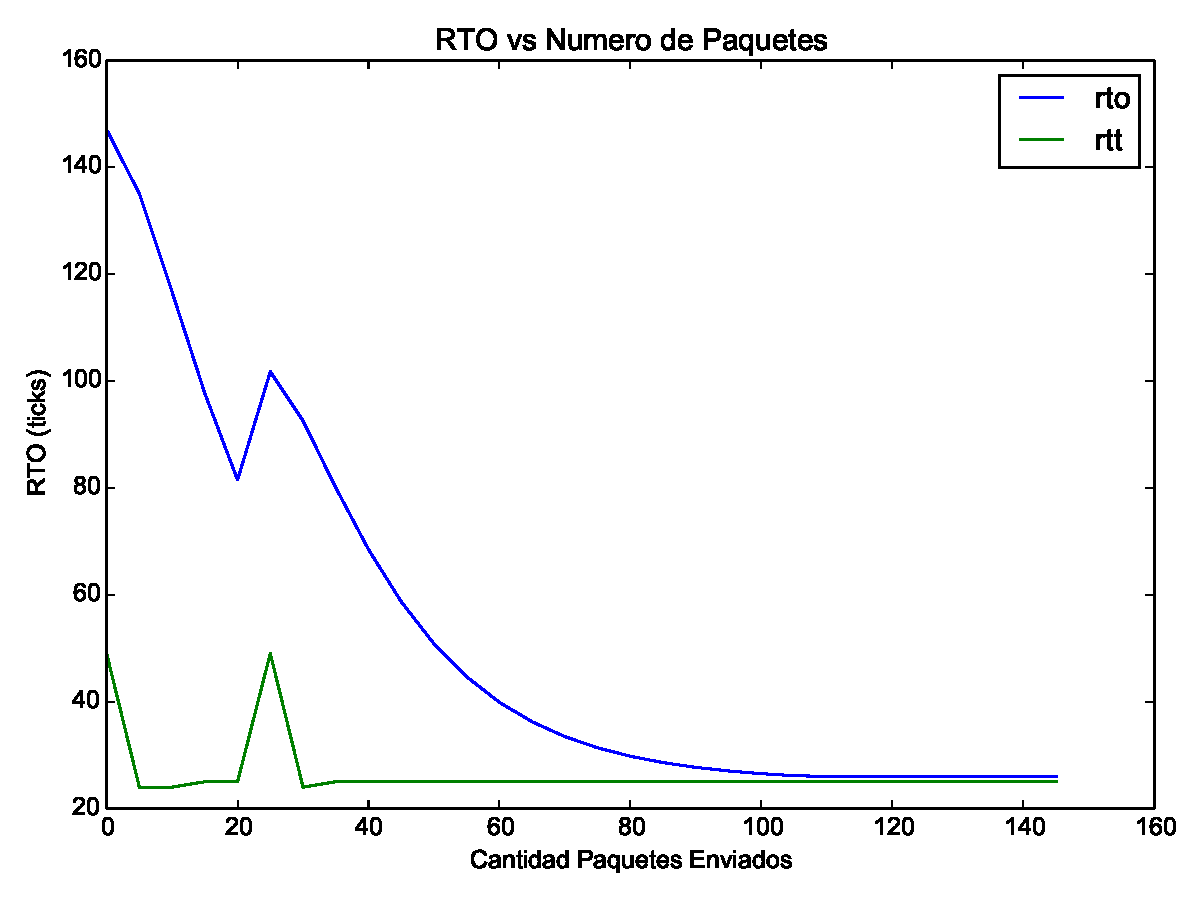
\includegraphics[width=0.32\textwidth]{imagenes/guille/rtt_vs_n_2_4.pdf}
		    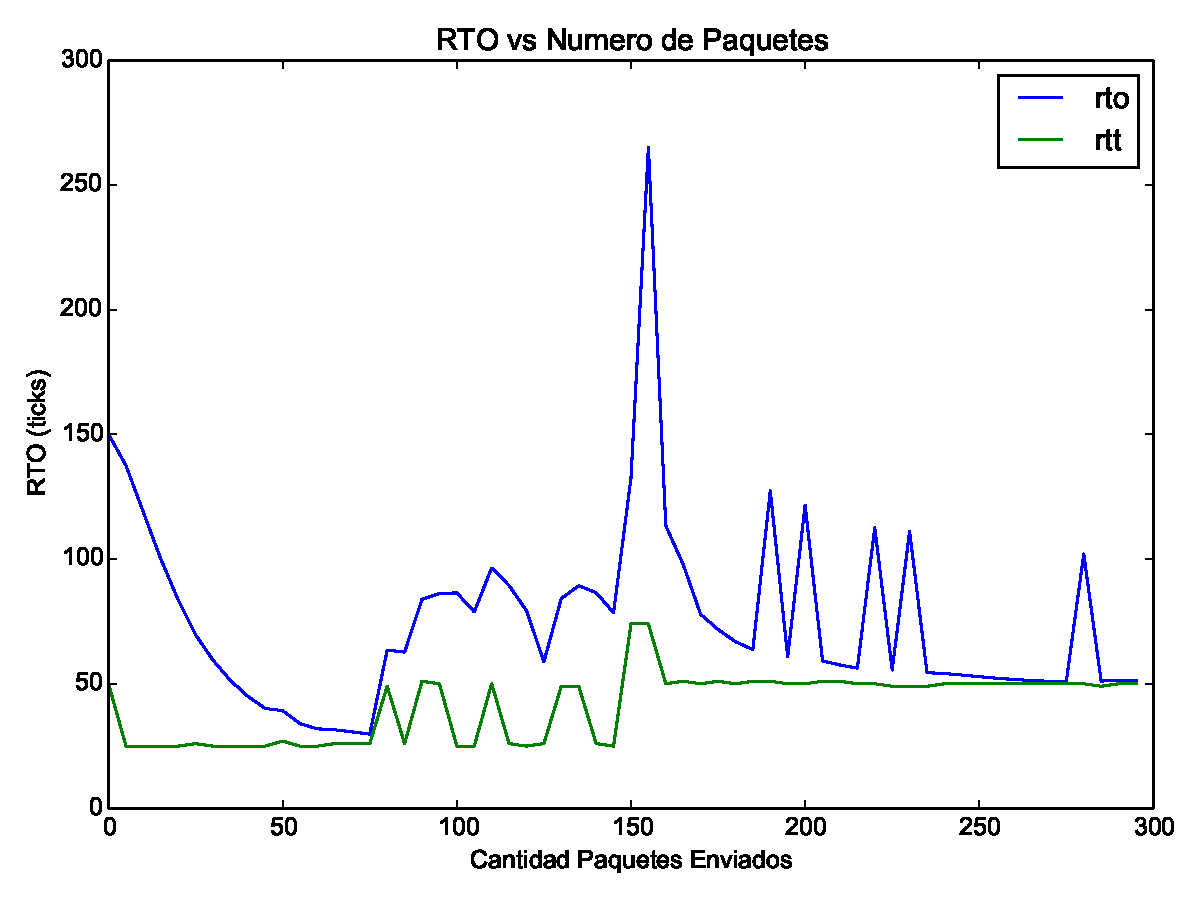
\includegraphics[width=0.32\textwidth]{imagenes/guille/congestion_50_2_4.pdf}
		    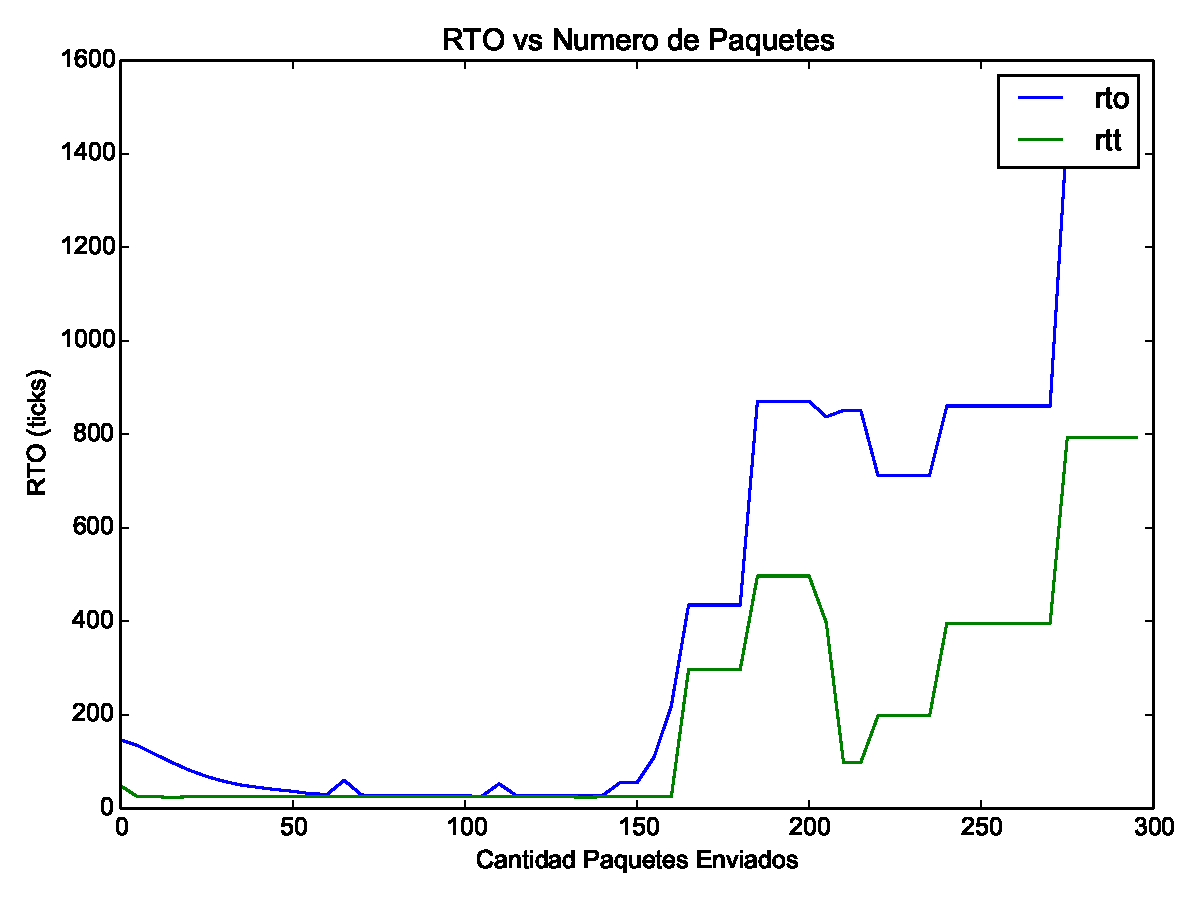
\includegraphics[width=0.32\textwidth]{imagenes/guille/congestion_100_2_4.pdf}

            \caption{Escenario 1}
	
        \end{figure}          
  
        El \emph{Escenario 2} muestra el resultado en una red con
        par\'aemtros: $\alpha={{1}\over{8}}$, $\beta={{1}\over{2}}$ 
        cuando no se congestiona, cuando la congesti\'on causa el doble de
        delay, y cuando causa el cuadruple.

        \begin{figure}[H]
            \center
	        
		    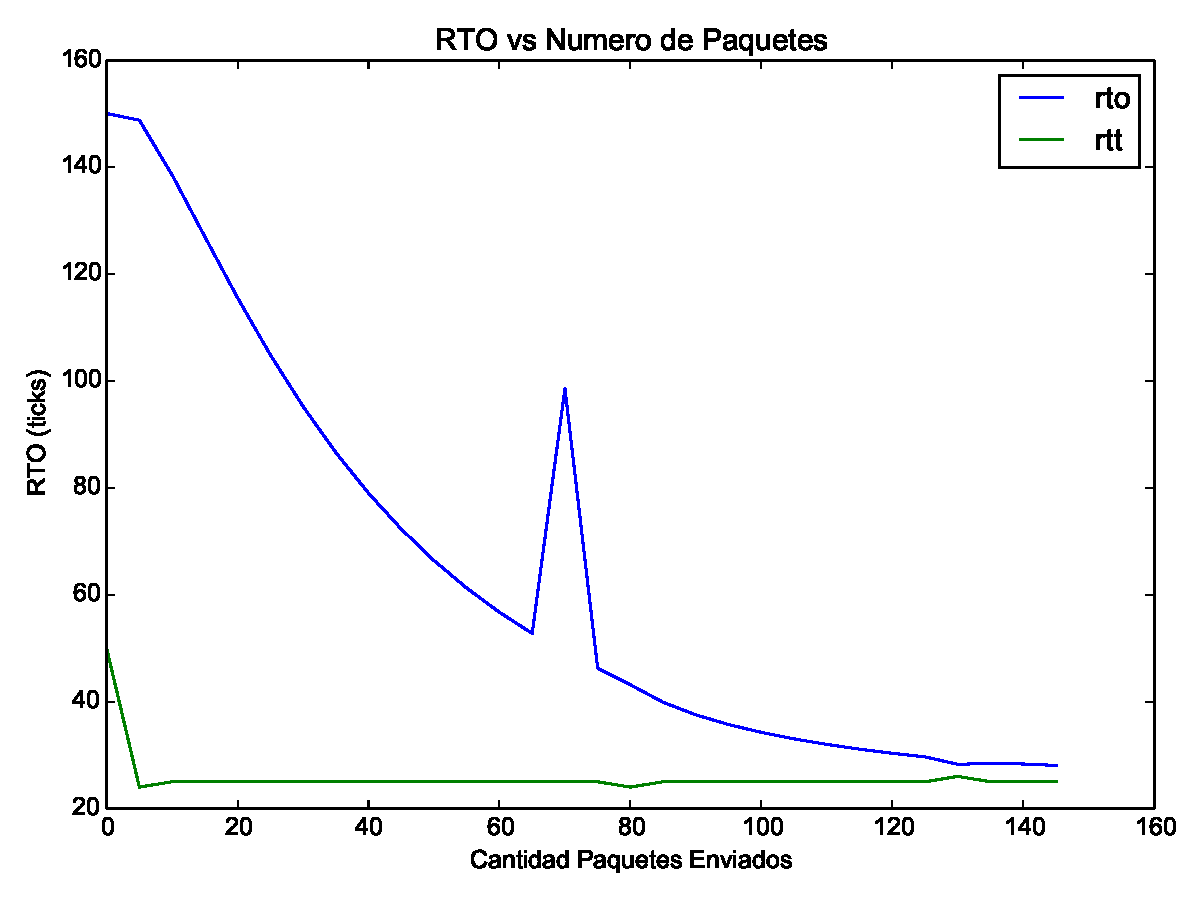
\includegraphics[width=0.32\textwidth]{imagenes/guille/rtt_vs_n_8_2.pdf}
		    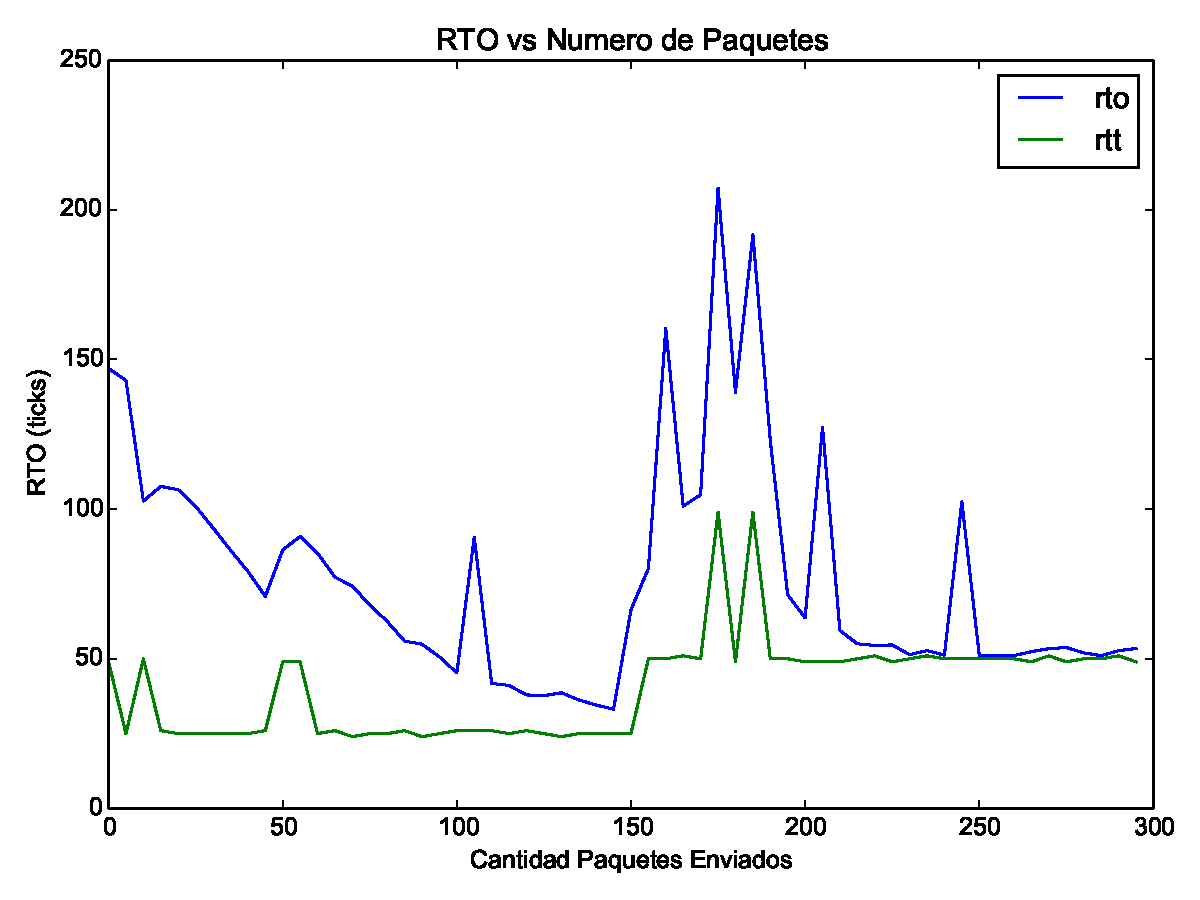
\includegraphics[width=0.32\textwidth]{imagenes/guille/congestion_50_8_2.pdf}
		    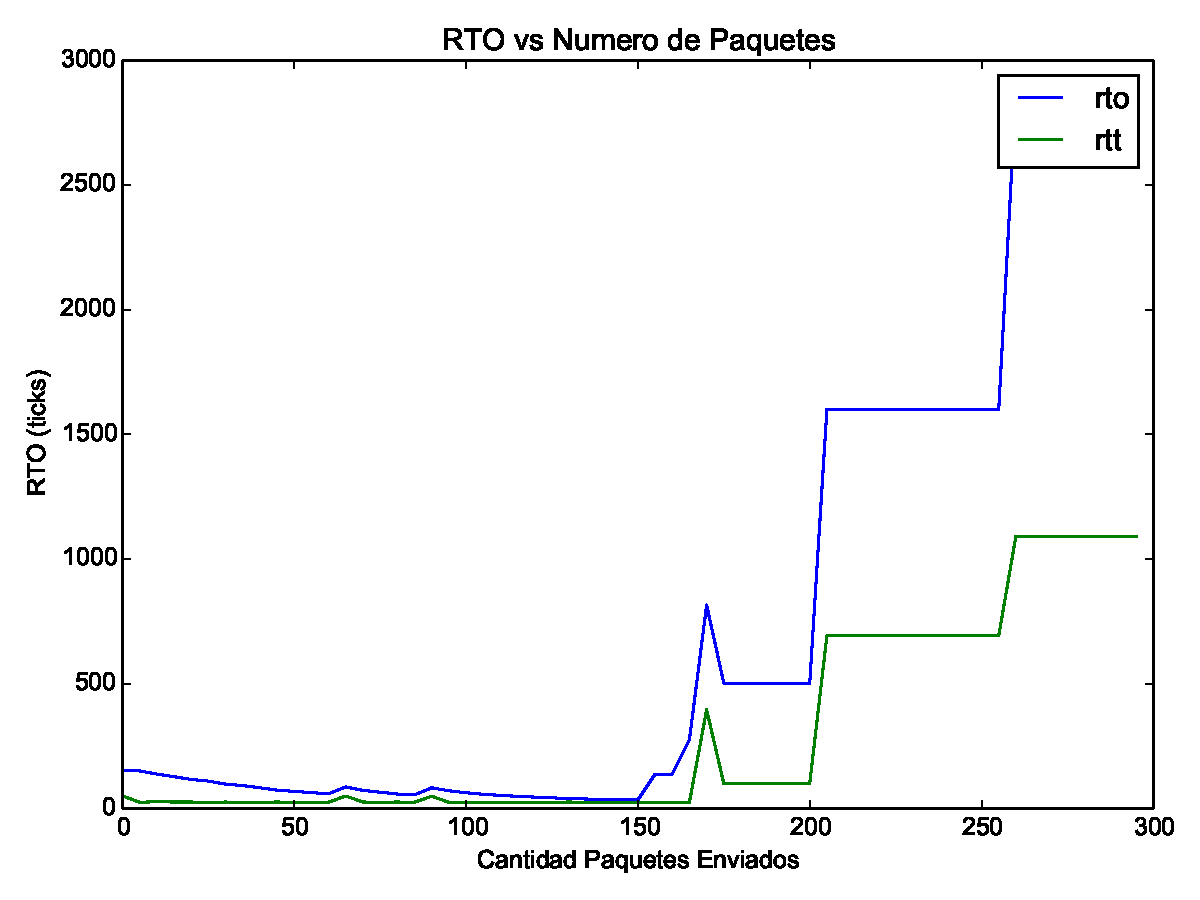
\includegraphics[width=0.32\textwidth]{imagenes/guille/congestion_100_8_2.pdf}

            \caption{Escenario 1}
	
        \end{figure}          

        En ambos casos sucedi\'o que al duplicar el valor del delay el 
        mensaje n\'umero 101 debi\'o ser retransmitido. A su vez, cuando 
        se cuadruplic\'o el valor de la red, el mensaje n\'umero 101 debi\'o
        ser retransmitido dos veces. 
        Tambi\'en se puede notar que en ambos casos luego de cuadruplicarse
        el delay no se logr\'o volver a un \rto{} cercano a el \rtt{} real.


